\documentclass[a4paper,english]{report}
\usepackage[utf8]{inputenc}
\usepackage{babel,duomasterforside}
\usepackage[backend=biber]{biblatex}
\bibliography{library.bib}
\usepackage{csquotes}
\usepackage{pdfpages}
\usepackage{graphicx}
\usepackage{mathtools}
\usepackage{amsmath}
\usepackage{amssymb}
\usepackage{subcaption}
\usepackage[nottoc,numbib]{tocbibind}
\usepackage{titlesec}
\titleformat{\chapter}{\normalfont\huge\bf}{\thechapter.}{20pt}{\huge\bf}

\begin{document}

\title{Thesis essay\\ [0.5cm]Modular Reinforcement Learning}
\subtitle{1st draft}
\author{Martin Jordal Hovin\\
\small 1st draft\\
[3cm]Supervised by:\\
Kyrre Glette}

\maketitle

\tableofcontents

\chapter{Introduction}
How is it a human brain is seemingly capable of learning an endless amount of tasks? Is it truly endless? Could we incorporate the same effect in our artificial minds?
    
Biology and nature have always been imitated in art and the sciences, but over the years the imitations are growing increasingly better. Artificial Intelligence and its sub-field of Machine Learning is one of these areas, and it is not bold to claim the ultimate goal of AI is to build what is referred to as \textit{General Artificial Intelligence}. A system capable of not only human-level performance in one field but able to generalize across domains and teach itself multiple new skills. 

In the quest for general artificial intelligence,  while there might be disagreement on what sub-fields of AI are the most important for this endeavor, improving on current learning systems is considered a good start\cite{mlroadmap}. The following pages will attempt to shed some light on some of the current state-of-the-art ideas and techniques applied to the fields of Reinforcement Learning, multi-task agents, and Transfer Learning. 

\section{Machine Learning}
How something is learned is something computer science have dabbled with since the days of Alan Turing, and have in the last decade seen an incredible surge of research activity. The field of Machine Learning (ML) is no longer a fringe topic but reaches all the way to the mainstream. 

In ML, the fields of statistics, mathematics, and data analysis are combined and applied to automate analytic modeling of data. A large number of algorithms and techniques exist in this domain of computer science, but the most current development and research are done on Artificial Neural Networks 

Inspired by the structure of the brain, the Neural Network (NN) consists of layers with any number of nodes within each layer. Such systems \textit{learn} to approximate a function based on the data we provide the network. Standard supervised methods work by the process of back propagation of an error metric and updating the weights of each node by \textit{gradient descent}. For some input, this error metric is reached by comparing the network's output to a \textit{ground truth} which is part of the training data.   

\section{Deep Learning}
While standard NNs have been used for a long time, the recent progress of machine learning can be attributed to the development of Deep Learning. Intuitively, the difference between NNs and Deep neural networks (DNN) is just the number of layers in the model, but functionally we can view the DNN as a collection of \textit{shallow} learning models, defined through the use of activation functions. Complex Deep Learning models have been effective at such tasks as image classification\cite{imageclassification}, natural language processing\cite{deepnlp} and Reinforcement Learning (see \ref{rlbackground}). 

Another common way of describing Deep Neural Networks is as Neural Networks which does its own feature extraction. A \textit{deep} Convolutional Neural Network (CNN)\footnote{Convolutional Neural Networks are models where weights are places in a kernel used during convolutions over some input. This is shown to be highly effective in image classification because of the deep CNN's ability to extract features which is scale and translational invariate.} for example, is able to abstract raw image input to a higher order feature representation which may be used in a fully connected layer for classification.
\begin{figure}
\centering
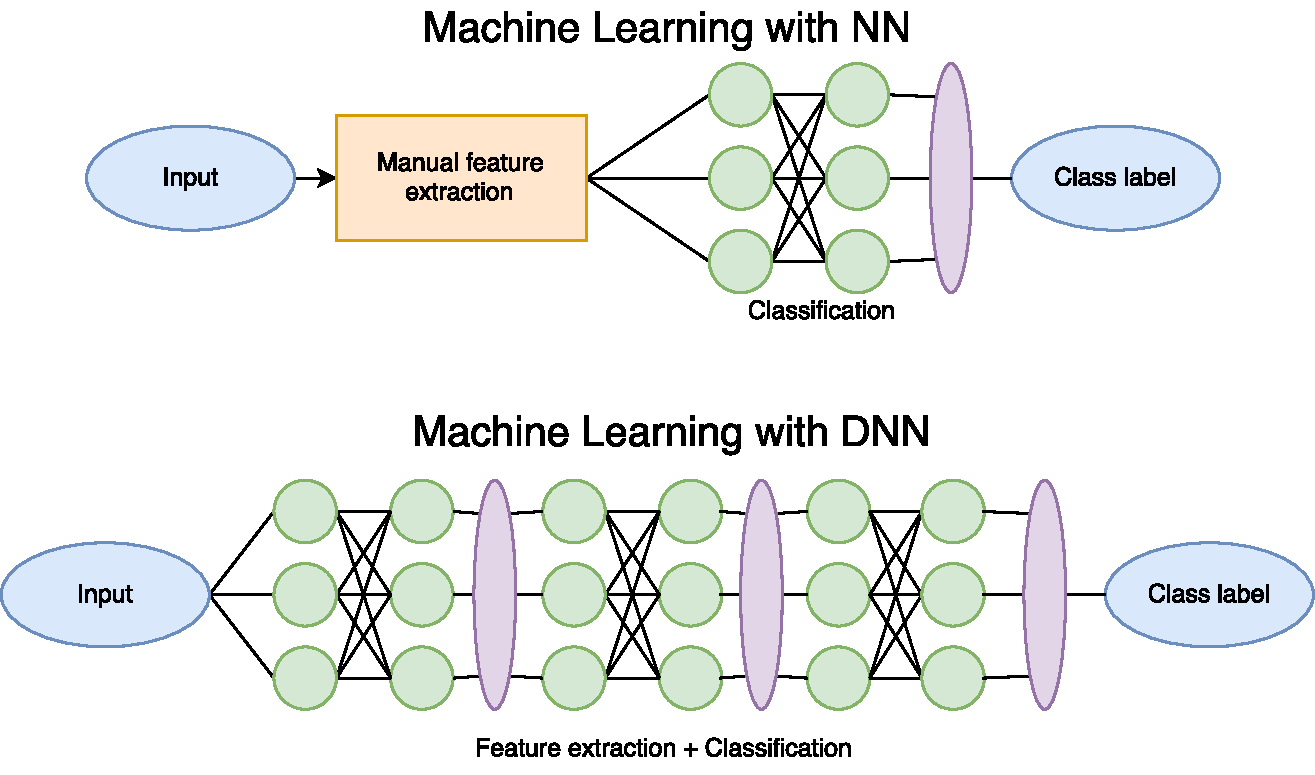
\includegraphics[width=0.8\linewidth]{figures/NNvsDNN.pdf}
\caption{Figure visualizes the difference between traditional Neural Networks and Deep Neural Networks. Note the addition of multiple activation layers (\textit{purple}) and the incorporation of feature extraction into the network itself in the Deep Neural Network}
\label{fig:NNvsDNN}
\end{figure}


\chapter{Reinforcement Learning}
\section{Background}\label{rlbackground}
While development of most machine learning and artificial intelligence systems are heavily inspired by biologic structures such as the brain, few algorithms are more relatable than Reinforcement Learning(RL). The learning is motivated by a stimulant given to an \textbf{agent} based on the actions taken. Much like one might train a dog by giving treats for a well-preformed task, we can train an artificial agent to perform actions we deem preferable. By providing positive rewards (carrots) for "good" actions and negative rewards (sticks) for "bad" actions, an agents behavior will converge towards the action scheme which tends to the highest reward (most carrots). 

The usual framing for a RL problem stems from its close connection to Markov decision problems (MDP) when it satisfies the Markov property\footnote{Every future state depends only of the current state, and not the previous.}. At a time step \textbf{t}, an \textbf{agent} observes an state \(s_t\) from a state space \(\mathcal{S}\). An action \(a_t\) is selected based on a policy scheme \(\pi(a_t|s_t)\), which is the agents behaviour. When the action is preformed the environment return a reward \(r_t\) and a new state \(s_{t+1}\). All sequential correlated states are considered part of the same episode, and the goal of a RL system is to preform actions which maximizes the total reward. What policy is used for the action selection varies from \textit{direct policy search} approaches such as \textit{evolutionary algorithms} and \textit{policy gradients} methods\cite{policygradient}, to approximation of value-functions such as \textit{Q-learning}(Watkins and Dayan, 1992).


\section{Reinforcement learning with Deep Neural Networks}
We achieve deep reinforcement learning by applying a deep NN as a function approximator on either a policy, a value function\footnote{Value describe how preferable an action was for a given state.}, or a state transition and reward model. Deep Reinforcement Learning with Q-learning\footnote{Such as the Deep Q-Network (DQN).} have lately proven capable of solving extraordinary complex tasks, even surpassing the level of expert human agents\footnote{Examples of this is games such as Go (Google’s AlphaGo\cite{alphago}, 2016), multiple Atari games (Google DeepMind\cite{DeepMindAtari}, 2014) and Dota2 (OpenAI\cite{dota2}, 2017).}. 

\subsection{DQN}
DQNs attempt to approximate the Q-function in an RL problem.
Given a state s and an action a, the update rule for the parameters \(\phi\) is at time step t+1 
\begin{equation}\label{eq:qlearningupdate}
\phi_{t+1} = \phi_t - \alpha(Q(s_t, a_t|\phi_t)-y_t)\nabla_{\phi_t}Q(s_t,a_t|\phi_t)
\end{equation}
where
\begin{equation}
y_t = r(s_t, a_t) + \gamma\max_{a}Q(s_{t+1},a|\phi_t)
\end{equation}
and \(r(s_t, a_t)\) is the reward associated with preforming action \(a_t\) in current state \(s_t\), \(\max_{a}Q(s_{t+1}, a_t|\phi_t)\) is the maximum total reward possible to achieve from the state reached as a result of  a, and \(\gamma\) is a scaling of future rewards\footnote{A value between 0 and 1 where 0 puts no value on future rewards, while 1 puts focus on the max total reward possible.}. The action \(a_i\) is chosen from a set of possible actions based on some policy \(\pi(a|s)\). Here \(\epsilon\)-greedy is a common scheme. Every action has a \(\epsilon\) probability of being random, and a 1-\(\epsilon\) probability of being \(arg\max_{a}Q(s_t, a_t)\). This is done to explore the state-action space. As the training progresses, we usually want to diminish this \(\epsilon\) value to focus the training to some optimized area.

\subsection{Dealing with problems}
The power of deep reinforcement learning is that it is able to learn abstraction of raw input without the aid of feature engineering. In a paper by Mnih et al.\cite{deepmindatariHumanlevelcontrol} a DQN was given raw pixel input from Atari games without any high-level features other than the reward signal. The paper found that their DQN out preformed humans in 29 out of the 49 games they tried.    
Under Q-learning implementation, sets of \(\{(s_i, a_i, s'_i, r_i)\}\) are collected. Depending on the implementation, these sets can be used directly to update \(\phi\) ("online" or "full fitted" Q-iteration), or stored in a replay buffer which is sampled later to avoid the problem of correlated sequential states. If this buffer is sampled in mini batches, the behavior distribution is averaged over many previous states, and feedback loops while training is mitigated.\cite{deepRLslide}

A a consequence of the max operator used in the update rule in \ref{eq:qlearningupdate} is overestimating the Q-function. Van Hasselt et al. \cite{doubledqn} proposed a Double DQN to handle this problem. Since the noice in \(Q(s',a'|\phi)\) and \(Q(s',a'|\phi')\) is decoupled, the overestimation can be avoided by using \(Q(s', arg\max_a Q(s', a|\phi)|\phi')\) instead of \(Q(s', arg\max_a Q(s', a|\phi')|\phi')\).

When compensating for the overestimating by the use of double DQNs, even better results were achieved on the Atari tasks than with the DQN proposed by Mnih et al.


\chapter{Transfer learning and Multi-task systems}
\section{Background}\label{tfbackground}
The approach of Transfer Learning (TL) is to use generalized knowledge in one domain as a basis for future learning in another. With the goal of achieving more effective learning in the target domain or even reaching a lower convergence point for the loss, TL shares some common ground with the field of multi-task learning, where the same model is applied to multiple tasks. 

We can define transfer learning as trying to learn a target conditional probability distribution \(P(Y_t|X_t)\) within a domain \(\mathcal{D}_t\), based on information gained from learning a source task \(\mathcal{T}_s\) in the source domain \(\mathcal{D}_s\) where \(\mathcal{D}_s \neq \mathcal{D}_t\) and \(\mathcal{T}_s \neq \mathcal{T}_t\). A domain \(\mathcal{D}\) would then, in a typical classification example, be given as \(\mathcal{D} = \{X, P(X)\}\) where \(X = x_1,x_2, \dotsc ,x_n\) are sampled from the feature space \(\mathcal{X}\) and \(P(X)\) is a probability distribution over that space. The task \(\mathcal{T}\) in that domain would then consist of a label space \(\mathcal{Y}\) and the conditional probability distribution \(P(Y|X)\) which usually is approximated during training on a set of \(x_i, y_i\) pairs where \(x_i \in \mathcal{X}\) and \(y_i \in \mathcal{Y}\).
\newline\newline
Traditionally, transfer learning has been applied in three ways: 
\begin{enumerate}  
\item Replacing the last layer in some trained NN. For example using the first layers of a CNN image classifier as feature extraction for some other image classification task 
\item Fine tuning a trained NN by restarting a back propagation sequence for new data from a domain \(\mathcal{D}_t\)
\item A combination of the preceding techniques where the last layers of a NN is replaced and trained from scratch, and the loss for these layers are back propagated through the rest of the already trained net.
\end{enumerate}
\subsection{Transfer Learning in CNN}
In a study by Yosinski et al. \cite{yosinski2014transferable}, results showed a transferability in the first layers of an image classifier during an experiment proposed to measure generality and specificity in the layers as transfer performance. The study divided the data set\footnote{The study used the ImageNet dataset of 2012 which contained 1,281,167 labeled training images and 50,000 test images, each labeled with one of 1000 classes.} in two random subsets (A and B), and trained two identical models on each of the subsets. Replacing the first n layers in two randomly initialized other models with the first n layers from the trained models (one from A, and one from B), they did an additional training step (fine-tuning by allowing back propagation through the copied layers in some cases) on data from subset B only. The goal was to study the effects transferring layers from one classification case to another had on accuracy. The best results reached were achieved when training a model on subset A, transferring the first three layers to a new randomly initialized model and fine-tuning these transferred layers while training the newly formed on data from subset B. 

\subsection{Catastrophic Forgetting}\label{catastrophicforgetting}
Not addressed by Yosinski is the problem of catastrophic forgetting, which is the effect that occurs when we fine tuning weights in a layer or NN which have been trained on a previous task. After fine tuning on target task \(\mathcal{T}_t\), the layer/NN may have forgotten how to perform the original source task \(\mathcal{T}_s\), depending on the extensiveness of the fine-tuning. This is not a problem unless the goal of the transfer learning is to train a multi-task system, where the source task \(\mathcal{T}_s\) is not considered just a step during training, but rather training for a task of the same importance as the subsequent tasks.

\begin{figure}[]
    \label{fig:ewc}
    \centering
    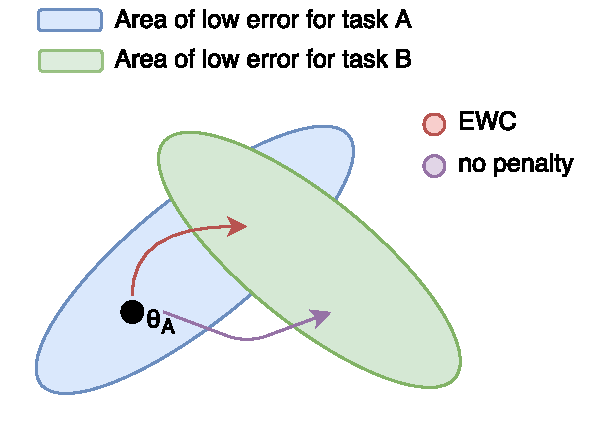
\includegraphics[width=8cm]{figures/EWC.pdf}
    \caption{Figure from the paper on reducing catastrophic forgetting\cite{ewc}. The figure shows the parameter space \(\mathcal{P}\) and hypothetical areas of low error for two tasks A and B. The arrows indicate the direction EWC\textit{red} and normal training \textit{purple} takes the parameters.}
\end{figure}
\label{section:ewc}
Efforts have been made to mitigate catastrophic forgetting in NNs during training of multi-task systems. Elastic Weight Consolidation (EWC) is a novel algorithm proposed in January of 2017 by Kirkpatrick et al.\cite{ewc}. During the transfer of weights from task A to task B, over-parameterization makes it likely that a solution to problem B\footnote{A solution may be viewed as a set of parameters \(\bar{\theta}\). Training a NN consists of adjusting these parameters through the process of back propagation with the gradient descent algorithm. For multiple parameters in \(\bar{\theta_A}\), many configurations of those values will give the same performance for the NN.} lay close to the solution for task A in the parameter space \(\mathcal{P}\). During optimization of \(\bar{\theta}\) for task B, EWC makes sure the parameters stay within an area of low error for task A.

Using EWC, Kirkpatrick et al.\cite{ewc} was able to train the same NN on 10 different Atari games without the effects of catastrophic forgetting between training tasks. With a human-normalized score of 1 for each game, giving a total possible score\footnote{where is 0 the same as a random agent, and 10 is at least human-level performance on all games.} of 10, the EWC driven training reached a score of around 6 after 500 million training frames, while the control never reached anything higher than 1.


\subsection{Curriculum Learning}
To guide an NN through a learning process, curriculum learning is a technique shown to work well. By gradually increasing the complexity of a learning task from simpler level until the desired complexity is reached, Bengio et al. \cite{curriculumlearning} was able to show a lower average test error and decreased convergence speed for multiple learning scenarios, as well as an increase in the quality of the local minima obtained.

\section{Progressive Neural Networks}\label{pnn}
Google DeepMind published a paper in September of 2016\cite{progressiveneuralnetworks} where they addressed the problem of catastrophic forgetting during transfer learning with fine-tuning. Their proposed solution, Progressive Neural Networks (PNN) were shown to be able to learn multiple tasks sequentially without overwriting the previously trained weights. This was done by horizontally scaling the DNN with a new stack of layers for each new task the PNN was applied to.

After training a DNN on a task A\footnote{In the paper, the PNN is focused as an application for Reinforcement tasks where the PNN were trained to provide probabilities over actions from a set of possible actions, from an input state.}, a new DNN were initialized randomly with lateral connections (see fig. \ref{fig:pnn}) to the NN trained on task A and then trained on task B with back propagation only done through the newly initialized layers. This ensures that the new DNN can optimize freely on task B, but will be able to utilize the weights trained on task A, without catastrophic forgetting occurring in the first DNN. When a sufficient performance on task B is reached, the PNN is able to perform optimally on both tasks, given some selection of the output (i.e: if given data for a task within the domain A, the output from the weights trained on task B is not optimal). Multiple tasks can be trained using this method. For each new task, a new DNN is initialized and the other DNNs in the PNN is connected laterally to each new layer. 

A problem with this scaling raised and addressed in the paper is that of quadratic growth of parameters for each new training task. Experiments show that there is a reduction in the new capacity actually utilized by the PNN for each new task added. This implies the growth of the PNN for each new task could decrease exponentially\footnote{Here the paper suggests pruning or online compression during learning.} without needing the new task to follow the same downward trend in complexity. 

Continual multi-task learning\footnote{The ability to accumulate knowledge provided along the lifetime of a model. This is regarded as the way humans learn.} may not be a solved problem, but PNN provides a stepping stone for future research on the topic. 
\begin{figure}[t]
    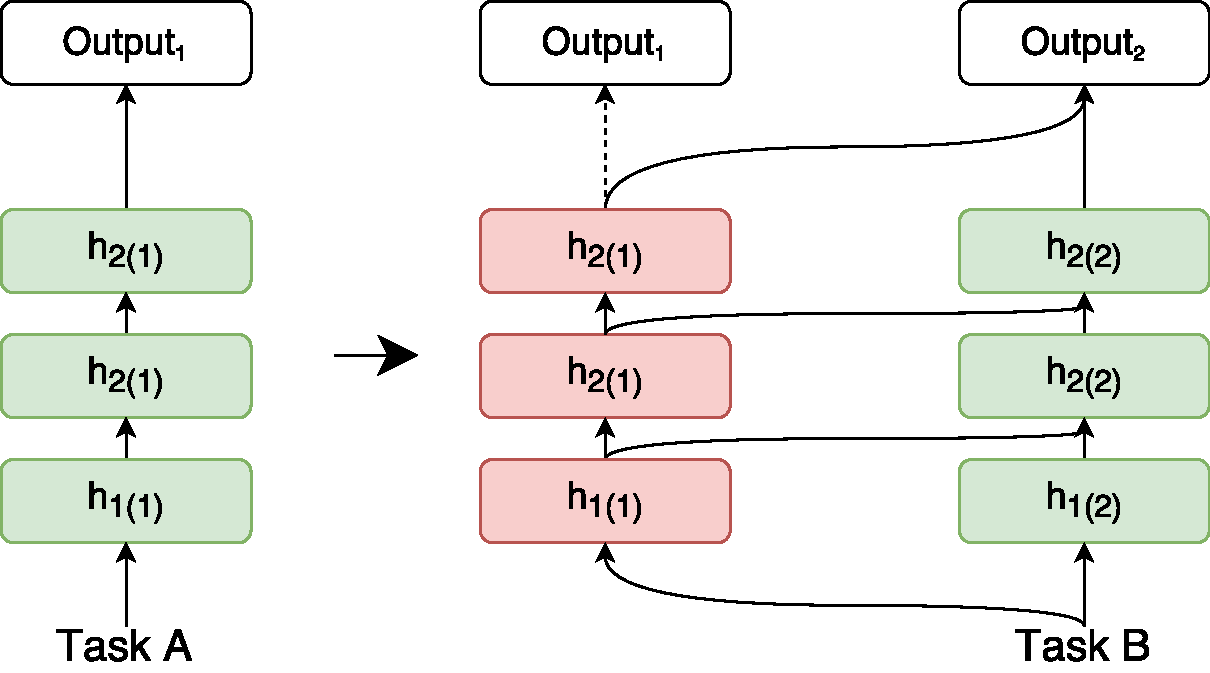
\includegraphics[width=\textwidth]{figures/ProgressiveNeuralNet.pdf}
    \caption{Example of a PNN. \textit{Left}: a three-layer NN is trained on task A. \textit{Right}: Adding another stack of three hidden layers that are being trained on task B. The weights in the first stack trained on A is now locked to the back propagation from task B, but its weights may be used is shown by arrows between the layers. Green indicates layer is open to back propagation, red indicates it is locked. The figure is a simplification of multiple figures from the article\cite{progressiveneuralnetworks}}
    \label{fig:pnn}
\end{figure}

\section{PathNet}\label{pathnet}
In 2017, DeepMind took the modular approach\footnote{Modular with respect to the traditional approaches of transfer from monolithic models} to deep transfer learning for multi-task systems one step further with their newly developed PathNet\cite{pathnet}. Where PNNs transfer knowledge between domains by adding new uninitialized DNNs for each task, the size of PathNet is not dynamic in the number of parameters. At training start, the net consists of randomly initialized weights in multiple DNNs, where each DNN is considered a module (or node) in a larger network of DNNs. 

Using a combination of evolutionary and machine learning techniques, PathNet shares the PNNs traits of being able to optimize for multiple training tasks without catastrophic forgetting and transfer knowledge between tasks by reusing locked weights.  

For each training task, a set of pathways through the network are initialized as phenotypes and evaluated through a set duration training period using gradient descent where all parameters along the phenotypes path are updated, and its fitness evaluated as a function of the loss through this path. Through a tournament selection algorithm, the variation in the genotype decrease and the set of paths converge on one optimal path through the net for the current task. The weights along this path are then locked to future back propagation, and all other weights are reinitialized randomly.
\begin{figure}[t]
    \label{fig:pathnet}
    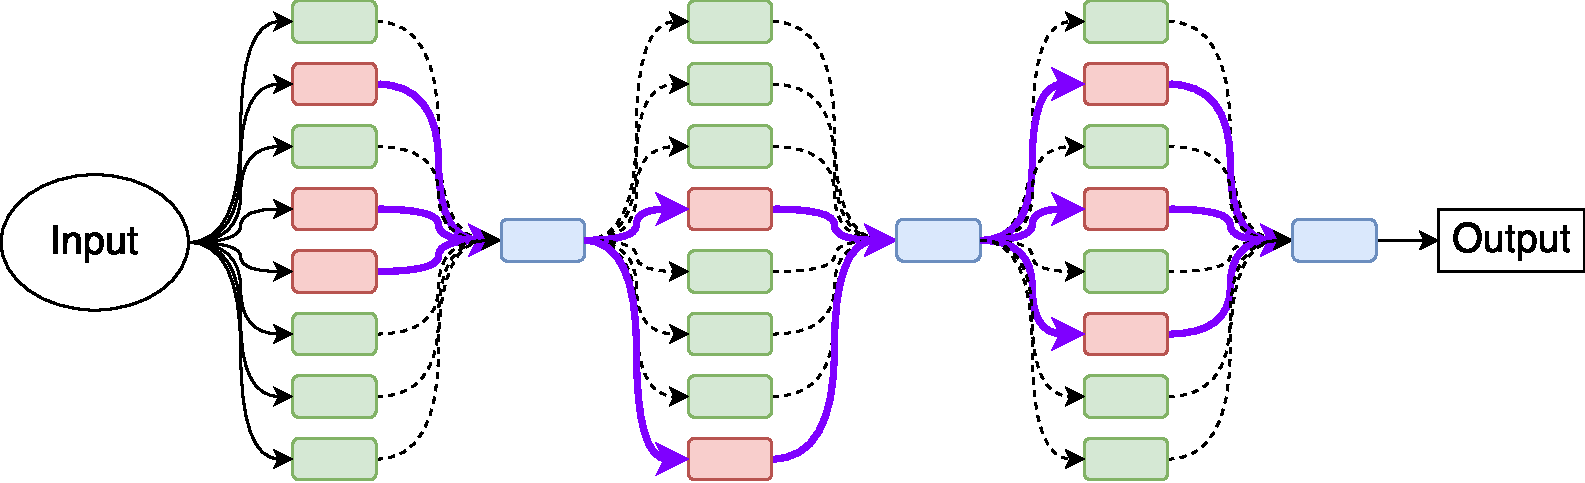
\includegraphics[width=\textwidth]{figures/PathNet.pdf}
    \caption{Figure shows a PathNet implementation with 3 layers of 8 modules (DNNs) in each layer. The \textit{red} color indicates the weights of this DNN is locked from back propagation, while \textit{green} indicates it is open. \textit{Blue} cells are reduced sum modules which summarizes the feature maps between each layer.The purple connections show a possible optimal path for a task. One path may use multiple modules from each layer.}
\end{figure}
This locking of parameters is the preventive measure that keeps fine-tuning of weights from destructively influence previously learned tasks but is also the limitation to number tasks the net is able to learn. As the number of tasks applied to PathNet increase, the number of locked parameters increase, and at some point, the net is locked from future learning. At that point, new knowledge would have to be encoded in the NN solely as a new path, and the algorithm responsible for this learning would, in the case of DeepMinds implementation, be the tournament search. The paper also states that other evolutionary techniques could be applied and even a RL-system, but this is not addressed.

While the process of evolving paths through tournament search alone might be a must for learning new tasks when the NN is fully locked, this might happen for a large net while some modules are still open. As the paper on PNNs showed, the capacity needed for new tasks diminish over a number of tasks learned if transfer learning is sufficiently achieved. Might a saturation point in a PathNet be reached, where previously gained knowledge saved in the modules may be used efficiently enough for new knowledge to be based on these modules alone? 

\chapter{Conclusion}
The thesis will look into how PathNet can be implemented in combination with a curriculum learning scheme for a locomotion task for some locked morphology. During training, optimal paths for each sub-task in the curriculum will be evolved, and as the training moves toward learning the final locomotion task, the paths will reuse more and more of previously optimized parameters. Advantages to this curriculum learning approach would be the gradual growth of the complexity of the task and apparentness of critical sub-tasks as they emerge.  
\newline\newline
Examples of interesting research questions to address during this work could be 
\begin{itemize}
\item Can we estimate the decline in needed capacity for each new sub-task learned from the curriculum?
\item Can similar\footnote{Similar tasks would be a slight change in morphology, or using the same morphology in a different environment(up-hill etc).} locomotion tasks be learned by only finding optimal path through the network and reusing locked parameters?
\item Could zero-shot learning take the form of an optimal path? 
\item Could such an reinforcement agent be trained in a simulation and transferred across the reality gap?
    \begin{itemize}
    \item Could the gap be bridged by the EWC(see \ref{section:ewc}) approach to loss calculation?
    \item Could applying the agent in the real world be viewed as another task along the task-manifold for locomotion, and be trained in the existing PathNet as another optimal path? 
    \end{itemize}
\item How would EWC during parameter optimization influence the learning?
\end{itemize}
The work could also include experimentation with different evolutionary or genetic algorithms in the search for optimal path through the PathNet. Recall that this was suggested but not addressed by Mnih et al. in \cite{pathnet}.


\cleardoublepage
\phantomsection

\addcontentsline{toc}{chapter}{Bibliography}

%Printing bibliography
%\newpage
\emergencystretch=2em
\printbibliography
\end{document}